\documentclass[letterpaper,11pt,twoside]{article}
\usepackage[utf8]{inputenc}
\usepackage{amsmath,amsfonts,amssymb,amsthm,latexsym}
\usepackage[spanish,es-noshorthands]{babel}
\usepackage[T1]{fontenc}
\usepackage{lmodern}
\usepackage{graphicx,hyperref}
\usepackage{tikz,pgf}
\usepackage{multicol}
\usepackage{fancyhdr}
\usepackage[height=9.5in,width=7in]{geometry}
\usepackage{fancyhdr}
\pagestyle{fancy}
\fancyhead[LE]{matematicas.german@gmail.com}
\fancyhead[RE]{}
\fancyhead[RO]{\url{https://www.autistici.org/mathgerman}}
\fancyhead[LO]{}

\author{Germ\'an Avenda\~no Ram\'irez~\thanks{Lic. Mat. U.D., M.Sc. U.N.}}
\title{\begin{minipage}{.2\textwidth}

\includegraphics[height=1.75cm]{Images/logo-colegio.png}\end{minipage}
\begin{minipage}{.55\textwidth}
\begin{center}
Taller 03, Función afín\\
Álgebra $9^{\circ}$
\end{center}
\end{minipage}\hfill
\begin{minipage}{.2\textwidth}

\includegraphics[height=1.75cm]{Images/logo-sed.png} 
\end{minipage}}
\date{}
\thispagestyle{plain}
\begin{document}
\maketitle
Nombre: \hrulefill Curso: \underline{\hspace*{44pt}} Fecha: \underline{\hspace*{2.5cm}}
\begin{multicols}{2}
 Ya sabemos que la función afín es de la forma
 \[y=mx+b\]
 donde $m$ es la pendiente y $b$ representa el punto en el que es interceptado el eje $y$. Si $b$ es cero, la función además es \emph{lineal}.
 \section*{Aplicaciones de la función afín}
 \subsection*{Ejemplo}
 El costo en pesos por hacer funcionar una bombilla de 60 watios está dado por la función $c(h)=9.0612h$ donde $h$ representa el número de horas que dura encendida la bombilla. Resuelva:
 \begin{itemize}
 \item[a.] ¿Cuál es el costo que se debe pagar por hacer funcionar una bombilla de 60 watios durante treinta días (un mes) tres horas diarias?
 \item[b.] Grafique la función $c(h)=9.0612h$
 \item[c.] Suponga que un bombilla de 60 watios funciona en un cuarto cerrado durante una semana hasta que una persona la descubre y la apaga. Utilice el gráfico de la parte b) para aproximar el costo de haber dejado encendida la bombilla durante una semana. Luego use la función para encontrar el costo exacto.
  \end{itemize}
 \subsubsection*{Solución}
 \begin{itemize}
\item[a.]  $c(90)=9.0612(90)=815.508$ Es decir el costo es aproximadamente ochocientos quince pesos con 51 centavos.
\item[b.] Ya que $c(0)=9,0612(0)=0$ y $c(100)=9.0612(100)=906.12$, se pueden usar estos dos puntos A(0,0) y B(100,906.12) para hacer la gráfica de la función ya que sabemos que es una recta con pendiente $m=9.0612$ y el punto de corte $b$ es 0.
\begin{center}
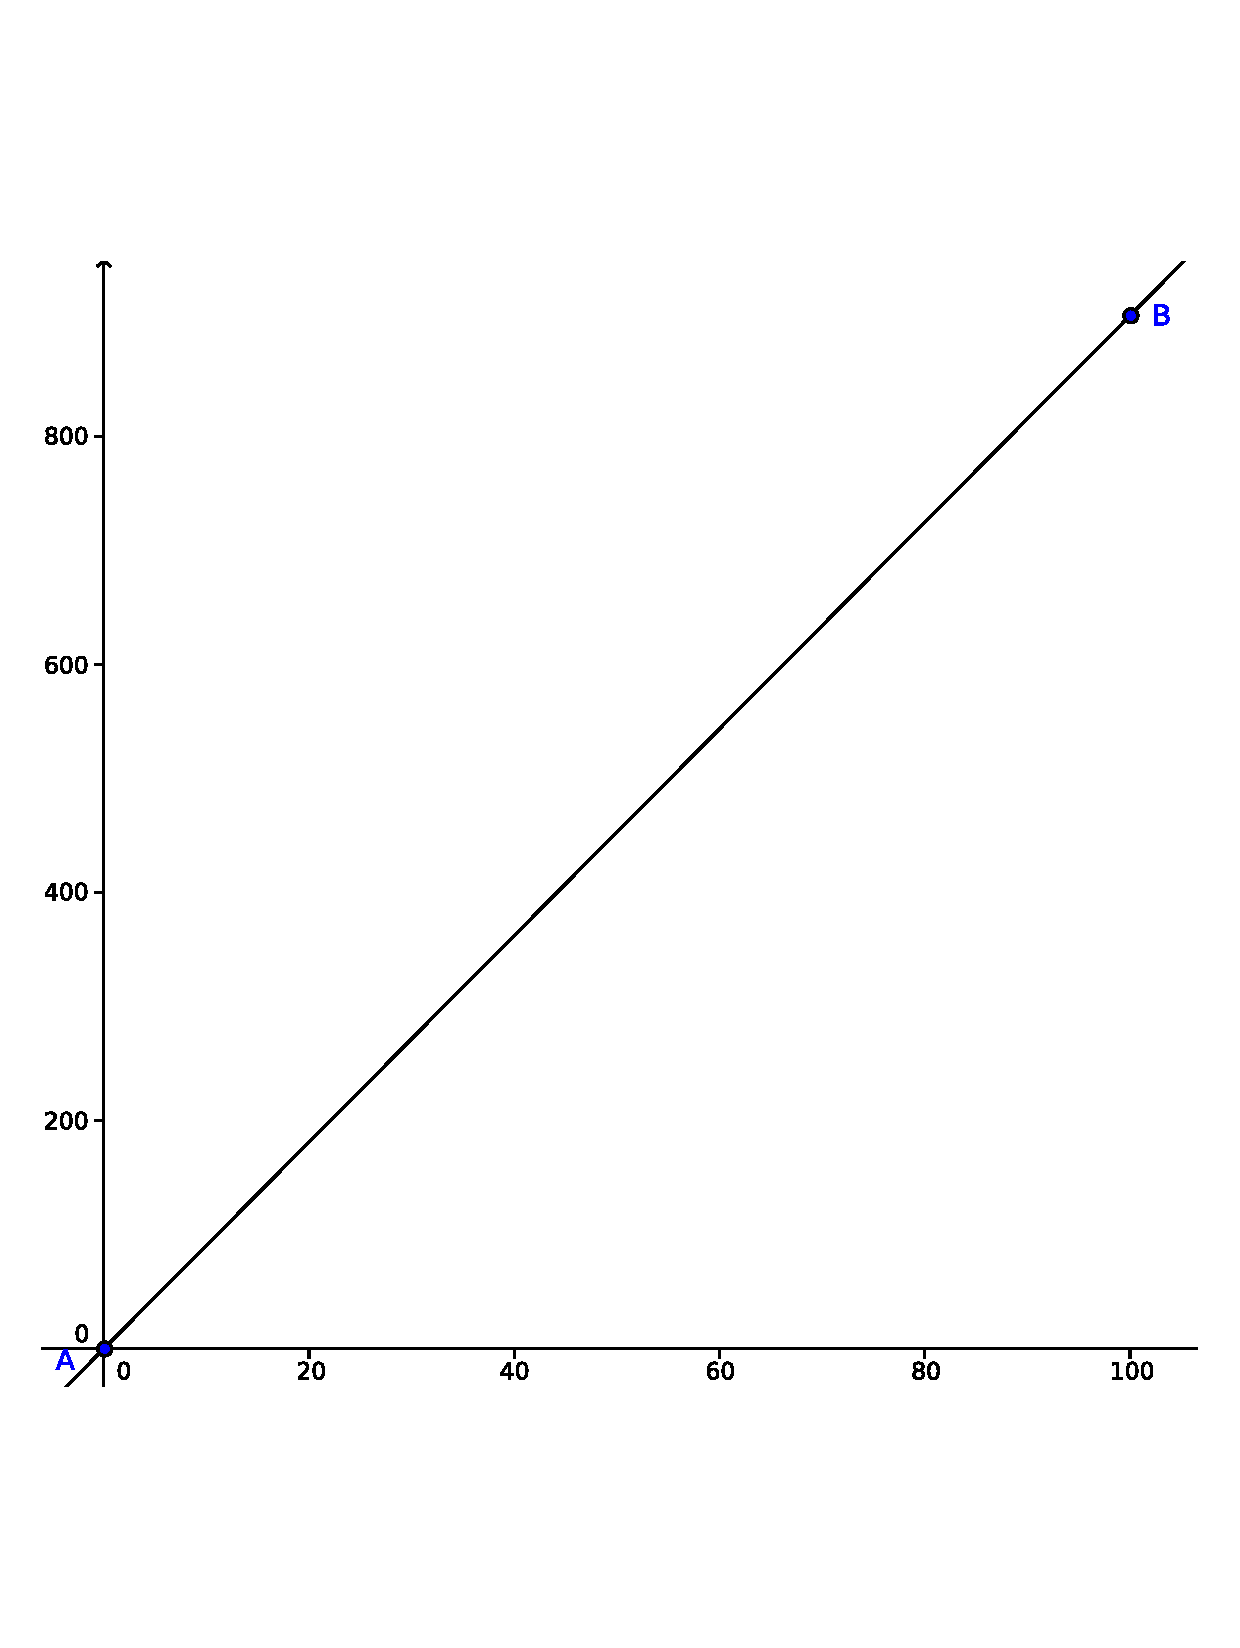
\includegraphics[trim=0cm 2.5cm 0cm 3.5cm, scale=.45]{Images/bombilla-graph.pdf} 
\end{center}
\item[c.] Si la bombilla dura encendida 24 horas al día durante una semana, esta dura $24(7)=168$ horas encendida. Con base en la gráfica se puede calcular aproximadamente cual es el costo; sin embargo la podemos calcular exactamente, usando su ecuación:
\[c(168)=9.0612(168)=1522.2816\]
es decir el costo de haber debajo el bombillo encendido durante una semana es \$1522.28 (mil quinientos veintidos pesos con veintiocho centavos)
 \end{itemize}
 \subsection*{Actividad}
 \subsubsection*{Quiz Conceptual}
 Para los siguientes items, conteste Verdadero (V) o Falso (F)
 \begin{enumerate}
 \item Cualquier función de la forma $f(x)=ax^{n}+b$, donde $a$, $b$ y $n$ son números reales es una función afín.
 \item Geométrica el valor de una función es la distancia directa del eje $y$
 \item La gráfica de una recta horizontal representa una función
 \item La función afín $f(x)=1$ es denominada la función identidad.
 \item Las gráficas de las funciones $f(x)=mx+b$ y $g(x)=-mx+b$ son perpendiculares
 \item Toda línea recta representa una función
 \item La ecuación $f(x)=ax+b$ también puede ser escrita como $y=ax+b$
 \item La gráfica de la función afín $f(x)=-4x+5$, es una línea recta con pendiente $-4$
 \end{enumerate}
 \subsubsection*{Problemas}
 Para los problemas \ref{ex01}--\ref{ex02}, grafique cada función afín
 \begin{enumerate}
 \begin{multicols}{2}
 \item $f(x)=3x+3$ \label{ex01}
 \item $f(x)=-2x+6$
 \item $f(x)=2x-6$
 \item $f(x)=-x-5$
 \item $f(x)=-4x$
 \item $f(x)=-1$
 \item $f(x)=\frac{2}{3}x+4$
 \item $f(x)=-\frac{1}{2}x-1$\label{ex02} 
 \end{multicols}
 \item Dada la función $f(x)=3x-2$, definida para todo $x\in \mathbb{R}$ encuentre $f(0)$, $f(2)$, $f(3)$, $f(-2)$ $-f(3)$
Para los problemas \ref{ex03}--\ref{ex04}, determine la ecuación de la recta para las condiciones dadas
\item \label{ex03} Determine la función afín para una gráfica que es una línea con pendiente $\frac{2}{3}$ y que contiene al punto (--1,3).
\item Determine la función afín cuya gráfica es una línea recta que pasa por los punto (--3,--1) y (2,--6)
\item \label{ex04} Determine la ecuación de la recta si su gráfica es una línea recta que es perpendicular a la función $g(x)=5x-2$ y contiene al punto (6,3)

Para los problemas \ref{ex05}--\ref{ex06}, aplique los conceptos de la función afín para contestar las preguntas
\item ~\label{ex05} Una empresa que alquila autos cobra \$35\,000 por día más \$550 por cada kilómetro recorrido. Determine la función que puede ser usada para calcular el costo diario de alquilar un auto. Ahora use la función para determina el costo de alquilar un carro durante un día conduciendo 140 km, 180 km, y 200 km.
\item Ober desea vender ciertos productos que le costaron \$120, \$230, \$650, \$1\,200 y \$1\,560 obteniendo una ganancia del 60\%. Determine la función que le permite ponerle precio a cada producto y luego utilícela para calcular el precio de venta de cada producto que el compró.
\item El costo de tener encendido un bombillo de 75 vatios está dado por la función $c(h)=12h$, donde $h$ representa el número de horas que funciona el bombillo.
\begin{enumerate}
\item ¿Cuál es el costo de funcionamiento de un bombillo de 75 vatios que funciona 3 horas diarias durante un mes de 31 días? Exprese su respuesta aproximando al peso más cercano.
\item Grafique la función $c(h)=12h$ \label{ex-b}
\item Use la gráfica de la parte ~\ref{ex-b} para aproximar el costo de usar un bombillo de 75 vatios durante 225 horas
\item ~\label{ex06} Use la ecuación $c(h)=12h$ para calcular el costo exacto por el uso de un bombillo durante 225 horas.
\end{enumerate}
\item Dibuje el cuadrilátero ABCD cuyos vértices son A(0,4), B(2,3), C(--1,--2) y D(--3,--1). Hallar las pendientes de los lados. ¿Cuáles lados tienen la misma pendiente? ¿Cómo son estos lados que tienen la misma pendiente?
 \end{enumerate}
 \end{multicols}
\end{document}
